%!TEX root =../MacbethThesis.tex
\acresetall
\chapter{Principled Operationalisation using Presage2}\label{ch:presage}

\lettrine[lines=3]{P}{rincipled} Operationalisation is the process of transforming a symbolic or formal representation of a system (often written in some kind of calculus) into a computer model of the system in question~\citep{Jones2013}. This process varies greatly in difficulty depending on the complexity of the system to be modelled and the requirements of the computer model. \marginpar{Should be citing something different here?} Models can range from small prolog programs~\citep{Pitt2005a} to significant software engineering undertakings~\citep{Timm2005}.

\ac{ABM} and \ac{MABS} are approaches to modelling and simulating complex systems as multi-agent systems~\citep{Macal2010,Moss2001}.
This is a form of micro-simulation, where by modelling low-level interactions from the `ground up' we can observe macro level behaviours such as self-organisation, self-adaptation and so on.
Simulation models are therefore composed of an environment or arena which models the behaviour of a physical or virtual world, and autonomous, intelligent `agents' who interact with this world and other agents. 
\citet{Axelrod1997} identifies the usefulness of \ac{MABS} as a means to understand social systems. 
This approach fits naturally to the principled operationalisation phase of the \ac{SIC} methodology, as we are observing desirable macro-level performance in social systems (which are multi-agent in nature), and aiming to reproduce this performance in a socio-technical system. 

It should be noted that principled operationalisation, \ac{ABM} and \ac{MABS} do not aim to create an exact model of a social or socio-technical system, particularly in regards to human behaviour. Both the \ac{SIC} methodology and \ac{MABS} methods stress the appropriate use of abstraction and/or compartmentalisation in order to simplify the model while being able to draw valid conclusions from the model's behaviour~\citep{Edmonds2001}.

Work in \ac{ABM} and \ac{MABS} has led to creation of many software packages and platforms to ease the development of simulation testbeds~\citep{CynthiaNikolaiandGregoryMadey2009}. These aim to reduce the engineering effort required to implement agent models, providing reusable components, user-interface based design and/or prescriptive frameworks. In particular, they aim to ensure simulation validity while maintaining usability and extendibility~\citep{Axelrod1997}.

In this chapter we derive a set of requirements for a general-purpose software platform for simulation of socio-technical systems, which is suitable for principled operationalisation. We then review a selection of existing platforms with respect to these requirements, concluding that building upon our existing Presage platform~\citep{Neville:2009} best meets our needs. Finally we present the result of this work, Presage2~\citep{Macbeth2014}. % TODO

%\section{Requirements}
%
%\begin{itemize}
%\item Heterogeneous agents
%\item Full agent architectures
%\item Inter-agent communication
%\end{itemize}

\section{Review of Software Platforms for Agent-based Simulation}\label{sec:p2:review}

There are many software tools and platforms available for the simulation of agent societies: A comprehensive survey by \citet{CynthiaNikolaiandGregoryMadey2009} includes 53 different toolkits. In this section we discuss the state of the art of \ac{MABS} toolkits and software platforms.

The afore-mentioned survey by \citet{CynthiaNikolaiandGregoryMadey2009} is an exhaustive survey of platforms documenting programming languages, software licenses, targeted research domains, presence of tutorials and support, and more for each platform. There are several other more focused reviews of simulation platforms: \citet{Railsback2006} describes and compares the implementation of several, gradually increasing complexity, models on four platforms, Netlogo, MASON, Repast and Swarm. \citet{Castle2006} reviews six platforms (Swarm, MASON, Repast, Starlogo, Netlogo and OBEUS) with a particular focus on geospatial simulations. \citet{Tobias2004} compares four platforms for `social-scientific' agent-based simulation (Repast, Swarm, Quicksilver and VSEit).

There are several reasons for using specific software tools for \ac{ABM} and \ac{MABS}, rather than bespoke software:
\begin{itemize}
\item \emph{Tools for non-programmers}---The inter-disciplinary nature of \ac{ABM} means than for many researchers software development is a major obstacle in adopting \ac{MABS}. Platforms can simplify model and agent implementation and hide complex implementation details, allowing more researchers to be able to understand and implement models without software engineering skills.
\item \emph{Rapid-prototyping}---The use of a platform precludes the need for work implementing and testing simulation control code when writing a software model. This time can be used for model implementation from the start, thus allowing researchers to very quickly of from ideas to working prototypes running in a simulation.
\item \emph{Code re-use}---An established platform providing a uniform base for the implementation of models and agent algorithm should allow for the porting of these implementations to other models and simulations. This enables collaboration as ideas can easily be adopted and compared without having to rewrite code.
\item \emph{High performance simulations}---Optimisation of simulations is a research area in its own right. Thus it is unrealistic to expect modellers to be able to write their own simulation software \emph{and} optimise it. The use of simulation platforms allows users to benefit from faster simulation performance.
\item \emph{Validation and verification}---Software engineering is an error prone activity. Using a known and peer-reviewed simulation platform affords some level of trust that this component should work correctly and not introduce false results. 
\end{itemize}

In this section we firstly derive a set of requirements and comparative criteria for agent-based simulation platforms. Using this we review a set of candidate platforms for principled operationalisation. 

\subsection{Requirements and Comparative Criteria}\label{sec:p2:reviewcritera}

% TODO paragraph test against software tool reasons + socio-technical reqs + principled op reqs.
We derive a set of review criteria based on a selection of relevant criteria from the previous reviews.

From~\citet{CynthiaNikolaiandGregoryMadey2009} we take generial criteria which affect platform uptake, usability and verifiability:

\begin{itemize}
\item Programming Language---The programming language required to use a platform has an affect on user uptake, quality of available development tools, code readability and succinctness, and ease of debugging~\citep{Railsback2006}. Use of custom programming languages my appear to limit the possible models which can be implemented on the platform, while general-purpose languages such as Java have known capabilities. These languages also come with a rich array of development suites to choose from to ease the development process.
\item Software License---Open source licenses are preferable as they allow the platform's code to be scrutinised, allowing both users and reviewers to verify that simulation output will be correct~\citep{Polhill2007}.
\end{itemize}

\citet{Castle2006} identifies criteria for ease-of-use:

\begin{itemize}
\item Required programming experience---Expertise needed in general programming and/or the language of the platform in order to correctly use the software.
\item Integrated charting/graphing/statistics---Whether graphical tools for data analysis during and after simulation are provided.
\item Tutorials/Documentation available---Presence of tutorials and documentation to allow one to train oneself to use the platform correctly and proficiently.
\end{itemize}

\citet{Tobias2004} provides several useful general criteria and criteria specific for the modelling requirements of socio-technical systems:

\begin{itemize}
\item Support for modelling---\ac{GUI} or other tools for reducing programming work and visualising output.
\item Support for experimentation---Tools for generation of simulations and data recording.
\item Large number of complex agents---The ability of the platform to efficiency run complex agents to intensive reasoning.
\item Inter-agent communication---The possibility of sending messages between agents, and for communication network topologies to be simulated.
\item Generating agent populations---Automatic generation of agent populations from input parameters or data.
\item Generating networks---Automatic generation of networks based on various characteristics.
\item Management of spatial arrangements---Ability to simulation situated agents.
\item Dynamically changing model structure---Whether the model can be changed during simulation execution.
\end{itemize}

We also add a final criterion specific to the principled operationalisation process:
\begin{itemize}
\item Rule engine---Executable specifications~\citep{Artikis2010} are formal characterisations where the calculus can be directly run as a computer model. These characterisations are declarative in nature, thus with a rule engine we can improve the speed and accuracy of principled operationalisation by directly integrating them into the simulation.
\end{itemize}

\subsection{Reviewed Platforms}

We will now review four software platforms with respect to the criteria we identified. These platforms are:
\begin{itemize}
\item Netlogo~\citep{Wilensky1999a}---This is a \ac{GUI}-driven modelling environment for simulating natural and social phenomena, aimed at ease of use for non-programmers. It uses a custom programming language for the specification of the environment and agent behaviours.
%\item JADE~\citep{Bellifemine2003}---This is a middleware for multi-agent system deployment which can also be used for simulation. It uses an agent model tied very closely to the FIPA agent communication specification\footnote{http://www.fipa.org}, and lacks support for modelling of the agents' environment.
\item Repast~\citep{North2013}---This is a familty of platforms created at the University of Chicago, originally based on the SWARM platform~\citep{Minar1996}. For this review we will look at their Java-based platform, Repast Simphony, which has superseded their other tools.
\item MASON~\citep{Luke2005}---This is a newer, discrete event, platform developed at George Mason University written in Java, and focusing on simulation execution speed.
\item Presage~\citep{Neville:2009}---This platform is a recent development, and therefore does not appear in reviews. It was developed specifically for simulation of social networks and dynamics but has found use in an array of other \ac{MABS} applications~\citep{Pitt2011,Carr2010} and features a strong animation and visualisation component.
\end{itemize}

% Notable omissions: SWARM and JADE

\autoref{tab:platformreview} shows the platforms rated according to the criteria we selected from \citet{CynthiaNikolaiandGregoryMadey2009} and \citet{Castle2006}. We will now discuss the remaining criteria:

\begin{table}
\begin{minipage}{1\textwidth}
	\myfloatalign
	\caption{Evaluation of simulation platforms according to review criteria}\label{tab:platformreview}
	\begin{tabularx}{\textwidth}{X|p{0.12\textwidth}p{0.12\textwidth}p{0.12\textwidth}p{0.12\textwidth}}
	Criterion & Netlogo & Repast & Mason & Presage \\ \midrule
	Programming Language & Netlogo & Java & Java & Java \\
	Software License & Closed source & BSD\footnote{Berkeley Software Distribution licence: A permissive free software licence. Not compatible with the \ac{GPL}} & AFL\footnote{Academic Free License: A permissive free software licence. Not compatible with the \ac{GPL}} & Closed source \\
	Required programming experience & Basic & Strong & Strong & Strong \\
	Integrated graphics & Yes & Yes & None & Some \\
	Tutorials / Documentation & Yes & Yes & Yes & No \\
	\end{tabularx}
\end{minipage}
\end{table}

\subsubsection*{Support for modelling}

This is the extent to which the platform speeds up common modelling tasks, for example by providing simple \ac{GUI}-based design and/or simple visualisation tools.

Being primarily \ac{GUI}-based, and including environment and graphing visualisation as standard, Netlogo performs well in this criterion. Similarly Repast has some \ac{GUI} tools, but still requires the majority of functionality to be implemented in code. The remaining platforms do provide helper classes for common tasks, but these still require implementation with code.

\subsubsection*{Support for experimentation}

This is how well the platform supports experimentation over multiple simulations to test parameter spaces. All platforms support parameterisation of simulation runs, however MASON and Presage lack the ability to automatically generate experiments consisting of a series of simulation runs.

\subsubsection*{Large number of complex agents}

None of the platforms impose a hard constraint on the number of agents in a simulation, though depending on the efficiency of the software, practical limits will be reached when either computational resources are exhausted, or the simulation takes too long to run.

Netlogo's simulation times have been shown to scale more with the size of the environment state to be modelled, while Repast and MASON scales with the number of agents~\citep{Railsback2006}.  However the agent models tested were fairly basic. More complex agent architectures are likely to be impossible in Repast. MASON is designed with the intention of accommodating complex agents by being fast and lightweight. Similarly Presage has been demonstrated simulating complex agents~\citep{Pitt2011}.

All but one of the platforms run their main simulation in a single thread. Repast uses a multi-threaded discrete-event scheduler to run some events in parallel, however this performance boost is only available to certain background tasks, and not appropriate for agent execution. MASON also allows for some parallelisation within a simulation step, which the users must add themselves. Thus these simulators have limited capabilities to exploit modern, multi-core processors.

There is, however, more options for scaling simulations to distributed architectures. The Repast developers also distribute a C++ platform for \ac{HPC} clusters~\citep{Collier2013}, but this is separate from the Java platform. There have also been several attempts to provide an automatic scaling of normal Repast models to \ac{HPC} clusters~\citep{Minson2008,Cicirelli2011}.
However, this work has yet to lead to the availability of easy scaling of models for these platforms, generally imposing some model limitations and requiring additional programming care in order to achieve a distributed simulation.

\subsubsection*{Inter-agent communication}

Repast supports basic exchange of data between agents. Presage supports more explicit message passing between agents. Netlogo and MASON do not support communication between agents, however some kind of data exchange could be implemented through modification of shared state values.

\subsubsection*{Generating agent populations}

All platforms support generation of agents from data and parameters. 

\subsubsection*{Generating networks}

Presage is able to simulation several types of dynamic network between agents, and these can be based on several agent characteristics. Similarly Repast is able to generate multiple network types. MASON and Netlogo do not explicitly support networks.

\subsubsection*{Management of spatial arrangements}

Repast, MASON and Presage support multiple spatial representations for the environment. Netlogo only has a grid representation.

\subsubsection*{Dynamically change model structure}

Repast and Netlogo allow for changes to agents and models during simulation execution. Presage and MASON do not (beyond what can be done with a Java debugger).

\subsubsection*{Rule Engine}

None of the platforms feature Declarative rule-engines as core features, however there have been some success in integrating rule-engines with Repast~\citep{Lotzmann2011}. 

\subsection{Summary}

From this review we see that the platforms considered here differ little in terms of features. The platforms all follow a similar pattern of `framework and library'~\citep{Railsback2006}, in which a framework for designing an \ac{ABM} is proposed and the platform is an implementation of this framework. Netlogo differs from the other platforms in its attempt to make model implementation simple for non-programmers, while trying to remain powerful enough for complex use-cases. The others require knowledge of Java in order to use. 

Repast performs the best over the evaluated criteria, however its lack of
explicit agent communication is problematic when dealing with complex, social
agents. MASON provides a more stripped down alternative, which is fast, but
requires that most advanced functionality be written from scratch. Being the
least mature of the reviewed platforms, Presage lacks in some areas,
particular documentation and user-friendliness. Its origins in the simulation
of social networks shows in its competence in agent communication---an
important aspect of socio-technical systems.

A major drawback, which all but Presage suffer from, is their permissive
handling of state. These platforms treat shared state as a public resource,
allowing reads and writes from all agents, with no limited accessibility.
While it is a reasonable assumption in most modelling scenarios that agents
will use this access correctly, there are problems from both modelling and
verification perspectives. We believe that, when modelling, it is preferable
to separate the agent logic from the logic updating environment state: The
agent logic decides what action to take, and the environment decides the
outcome of that action. The architectures of Netlogo, Repast and MASON put
these two processes together, such that in order to take an action the agent
must update the environment itself. Presage uses separate \emph{action
handlers} which process actions from agents in a uniform and consistent way.
This ensures that the environment is the same for all agents, that agents are
portable between different environments, that agents can be unknowledgeable
about the consequences of actions they perform, and that faulty agent code
won't break a simulation.

It is for this reason that we decide to build on the promising  framework of Presage and address its shortcomings in a new version, Presage2. We describe the design and implementation of this platform in the next section.

%The core of a multi-agent simulation is a fairly straightforward control process. There is some representation of the environment state and of the state of agents in the environment. 

% middleware vs pure simulation platform

% discrete time vs event vs continuous

\section{Presage2 Platform}

In the previous section we outlined the need for a simulation platform for
principled operationalisation, and, through a review of existing platforms,
identified that the Presage framework was best suited to the task. In this
section we, firstly, describe the framework of Presage2, an evolution of the
original Presage, secondly, describe its implementation as a Java library,
and, finally, evaluate it with respect to the criteria in the previous
section.

\subsection{Framework Description}

The Presage2 framework is a result of an iterative improvement to that of the
original Presage framework~\citep{Neville:2009}. We build on the same concepts
in order to achieve the desired feature-set.

At its core, the framework uses a discrete-time driven simulation loop. This
is similar to the discrete-event models used in platforms such as MASON and
Repast, except that every agent is given the opportunity to submit actions at
each discrete time-step. This method establishes a minimum unit of time within
the simulation which is equal for all agents. The drawback of a discrete-time
approach is that the simulation cannot optimise periods when agents want to
wait several time-steps with no action, which is possible with discrete-event
simulators. However, in practice, this performance hit is negligible as,
firstly, most agents have reactive components which require constant
monitoring of the environment state, and secondly, a waiting agent can simply
return immediately when queried for actions by the simulator, wasting very
little resources. The advantage of time-driven over event-driven simulation is
that the former is easier to parallelise~\citep{Ferscha1995}.

Beyond the discrete-time driven constraint, the framework does not specify how
agents should be implemented, or what architecture they should use. There are
many possible architectures which can be used for agents to define their
\emph{agent function}~\citep{Rao1995,Kakas:2004bh}. The platform simply
queries for the result of this function each time-step. To support operating
at multiple levels of granularity, and to handle cases when agents are able to
perform multiple actions at once (for example a communicative action could be
performed at the same time as a physical action), we allow multiple actions
per agent per time-step.

The state of the environment and observable state of agents (i.e. state which
can be perceived by other agents), collectively referred to as \emph{shared
state}, is updated each time-step by a function we call a \emph{state
transformer} function. This takes the current state and set of agent's
actions as input, and creates the next state. This state change may be 
\emph{non-deterministic} with the addition of randomness. State changes may 
also be applied independently of an action. Note, however that the state change 
is transactional---all changes for one time-step are applied atomically. This
makes the environment \emph{static} for agents, and means that the result of
an action is not observable until the following time-step. Furthermore, it allows 
for deterministic state transitions, even when the execution order of agents 
cannot be guaranteed.

While the \emph{shared state} of the simulation can be made entirely
\emph{accessible} to agents, in most practical systems agents will not have
full observability or omniscience. Each agent instead has a partial view into
the shared state. This may be simply a subset thereof, or it could provide
modified values to simulate lossy or faulty sensors. Thus we can model
arbitrary levels of accessibility for each agent in the simulation.

This state model implicitly enables inter-agent communication of arbitrary
data between agents. A message action can simply create a state value which is
only accessible to the intended receiver agent. This action may also fail
randomly, if the agents are physically situated too far from each other, or due
to any other deterministic or non-deterministic factors relating to the environment
state. Therefore, we can model agent communication networks of arbitrary
complexity.

%With the described framework we can formalise a modelled system following the abstract architecture specified in \citet{Wooldridge2002}.

With the described framework we can formalise a modelled system as a four tuple:
\begin{equation*}
\mathcal{M}_{t}=\left\langle \mathcal{A},\epsilon,\tau,\phi \right\rangle _{t}
\end{equation*}

Where $\epsilon$ is the environment state, $\mathcal{A}$ is the set of agents, $\tau$ is the state transformer function and $\phi$ is the state observability function. Each
agent $a\in\mathcal{A}$ has internal state $s_{a,t}\cup s_{a,t}^{\prime}$,
where $s_{a,t}$ is public and $s_{a,t}^{\prime}$ is private, and
an agent function $f_{a}$. This function maps the agent's state and his observation of the environment and agents' public states (calculated with the state observability function $\phi$) to a private
state for the next time-step, $s_{a,t+1}^{\prime}$, and a set of actions
$H{}_{a,t}$:
\begin{align*}
f_{a}:\; s_{a,t}^{\prime} \times \phi(a, \epsilon_{t}, S_{t}^{\mathcal{A}}&) \rightarrow\; H_{a,t}\times s_{a,t+1}^{\prime}\\
S_{t}^{\mathcal{A}}&:=\bigcup_{a\in\mathcal{A}_{t}}s_{a,t}
\end{align*}

The state transformer function $\tau$ defines how the set of all
agents' actions $\mathcal{H}_{t}$ for a time-step map the current
environment and agents' states to new values for the next timestep:
\begin{align*}
\tau:\;\mathcal{H}_{t}&\times\epsilon_{t}\times S_{t}^{\mathcal{A}}\;\rightarrow\;\epsilon_{t+1}\times S_{t+1}^{\mathcal{A}} \\
\mathcal{H}{}_{t}&:=\bigcup_{a\in\mathcal{A}_{t}}H_{a,t}
\end{align*}

In his abstract architecture for intelligent agents, \citet{Wooldridge2002}
defines a \emph{run} for an agent as a sequence of interleaved environment
states and actions. Here we can do the same, but expressing that in our
framework the state is a \emph{view} of the system's \emph{shared state}, and
that an agent may have a set of multiple actions between consecutive states:
\begin{equation*}
\phi(a, \epsilon_{0}, S_{0}^{\mathcal{A}}) \xrightarrow{H_{a,0}} \phi(a, \epsilon_{1}, S_{1}^{\mathcal{A}}) \xrightarrow{H_{a,1}}  \ldots \xrightarrow{H_{a,u-1}} \phi(a, \epsilon_{u}, S_{u}^{\mathcal{A}})
\end{equation*}

Additionally, we can express a simulation in this way, as interleaved \emph{
shared states} and sets of actions:
\begin{equation*}
(e_0, S_{0}^{\mathcal{A}}) \xrightarrow{\mathcal{H}_{0}} (e_1, S_{1}^{\mathcal{A}}) \xrightarrow{\mathcal{H}_{1}} \ldots \xrightarrow{\mathcal{H}_{u-1}} (e_u, S_{u}^{\mathcal{A}})
\end{equation*}

% randomness; environment change; non-deterministic-ness

\subsection{Software Design and Implementation}

This framework purely specifies what can be implemented, and how state should
be controlled. There are many other criteria for a platform beyond this, as we
outlined previously. In this section we describe how this framework is
transformed into a platform architecture and an implementation in Java.

Our framework states that a simulation consists of four components: a set of
agents, an environment state, a state transformer function, and a state
observability function.  In order to support modularity and component reuse in
the platform we decompose the monolithic functions to provide units of
functionality. The state observability function is split into a set of
functions, named \emph{environment services} providing high level access to
shared state, while also defining observability. The state transformer
function consists of two sets of functions: firstly a set of \emph{action
handlers} which define state changes for specific actions, and secondly, a set
of \emph{environment} functions which define general state changes, for
example for persistent effects on agents (momentum or current), or periodic
(either random or triggered) events.  As we do not constrain the agent
architecture, the agent function is not decomposed. Through specification of
these sets of components one can define arbitrarily complex environments.
Furthermore, components can be bundled together into `modules' which provide
specific functionality.

The state of the environment, and public state of agents (\emph{shared state})
is managed by a state engine. This acts as a low-level state-data store which
other components use to access state values and commit state changes. It
provides a read-only interface to fetch data as well as an interface to
specify what changes should be made to the state at the end of the time-step.
The aggregated state changes are then all executed in a single transaction.
Thus it is impossible for agents to read a future state of the system.

As we have stated, \emph{environment services} provide high-level access to
the environment state. By this, we mean the service can provide a more rich
representation of the raw state data. This could be, for example, searching
the state of neighbouring cells in an environment and returning a list of
nearby agents. The service can also simulate partial observability of the
state by returning limited or modified results from these queries.

Conceptually, these \emph{environment services} simulate the behaviour of a
perception device for an agent. In a real-world scenario an agent would have
some interface for perceiving the state of the environment. By using this
abstraction we aim to enable the writing of agents who are not tied too closely
to the simulation platform, and whose simulated perception can be easily
replaced with real perception for rapid transition from simulation to
deployment.

\begin{figure}
\caption{UML Sequence diagram of interactions with shared state in Presage2}\label{fig:p2envsequence}
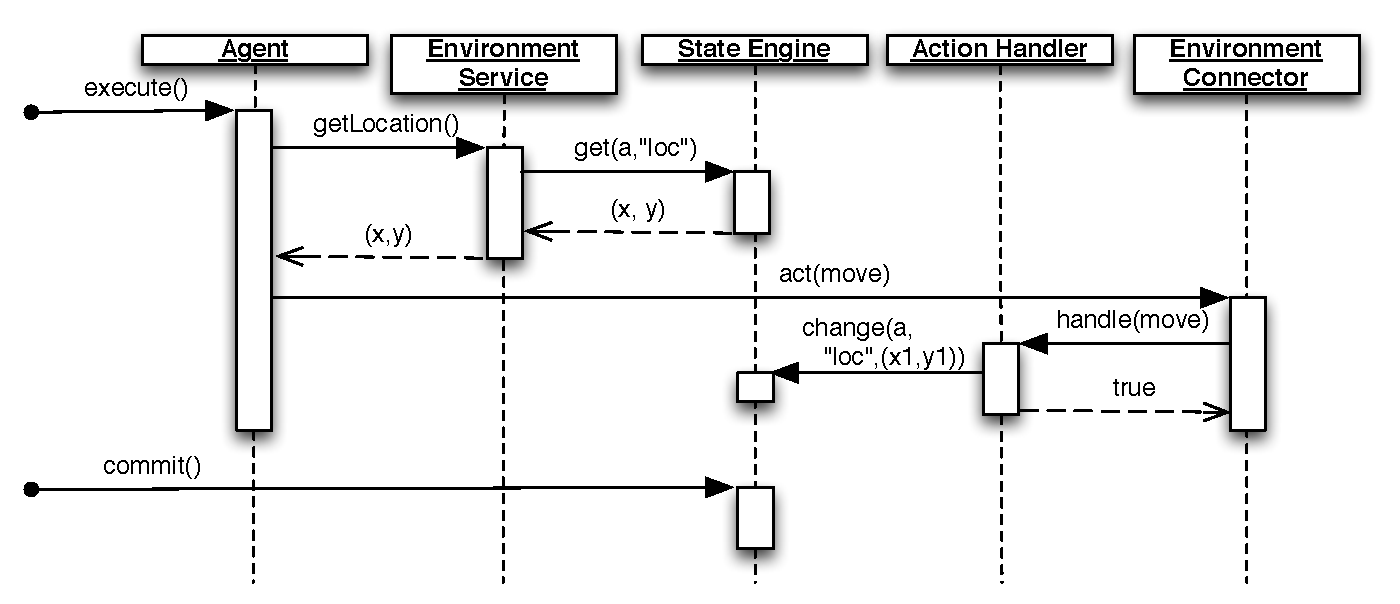
\includegraphics[width=\linewidth]{gfx/presage2/environment_sequence}
\end{figure}

\autoref{fig:p2envsequence} shows the interactions between environment
service, action handler and state engine for an example scenario. When an
agent is invoked by the simulation scheduler he can retrieve his state (in
this case a location) via an environment service. This service, in turn,
queries the state values from the state engine and returns them to the agent.
Using this information the agent chooses to do a `move' action, submitting it
via its environment connector (a simple interface used to perform actions).
This connector then chooses an action handler for this action, and a state
change is submitted to the state engine. Note the state is not actually
changed until the engine is instructed to commit changes at the end of the
time-step.

An example of how this would be implemented in an agent is shown in
\autoref{alg:agentimpl}. The \texttt{AbstractParticipant} base class provides
a useful base for the implementation of agents in Presage2. For example,
fields in the agent class of type \texttt{State} provide a dynamic binding to
an agent's state, via the appropriate environment service, and the
\texttt{act} function submits agent actions to the environment. The
\texttt{@Step} annotation designates which function(s) in the class are agent
functions. In this case, the agent function reads the agent's current
location, then constructs a move action to a target location and submits it to
the environment.

\begin{java}[caption={Presage2 agent implementation},label=alg:agentimpl]
class Agent extends AbstractParticipant {
	public State<Location> location;

	Agent(String name, Location initial) {
		super(name);
		this.location = new State<Location>("location", initial);
	}

	@Step
	public void step(int t) {
		Location loc = location.get();
		// calculate move to get to target from current
		Move m = getMove(loc, target);
		this.act(m);
	}
}
\end{java}

The final component required to implement the Presage2 framework is a
simulation loop to execute these functions correctly. The use of a immutable
shared state during a time-step simplifies this process, as state cannot be
corrupted by out-of-order operations. As we show in
\autoref{fig:p2envsequence}, environment services are triggered by requests
from agents, and similarly, action handlers are triggered by actions.
Therefore at the top level the simulation scheduler simply must invoke all
agent and environment functions. Once these tasks have completed the state
change is committed.

This process is parallelised on multi-core processors by running agent and
environment functions in parallel using a thread pool. This is a pool of
threads available to which tasks can be submitted. The pool manages the
allocation of tasks across the threads in the pool to optimise resource
utilisation\footnote{We use the \texttt{ThreadPoolExecutor} implementation
provided in the Java libraries.}. This enables multi-threaded simulation which
is transparent to the model implementer.

\autoref{alg:simloop} shows this simulation loop. Note object types and function names have been changed for illustrative purposes.

\begin{java}[caption={Presage2 multi-threaded simulation loop},label=alg:simloop]
do {
	for(Agent a : agents) {
		threadpool.submit(a);
	}
	for(Function f : environmentFunctions) {
		threadpool.submit(f);
	}
	threadpool.waitUntilComplete();
	stateEngine.commit();
} while(checkFinishCondition() == false);
\end{java}

The platform as a whole consists of several components, as shown in
\autoref{fig:presage2block}. We have already described the state engine, and
the simulation loop which is part of the core simulator. We will now introduce
the remaining components which bring an array of different features to the
platform.

\begin{figure}[tb]
\caption{Presage2 architectural block diagram}\label{fig:presage2block}
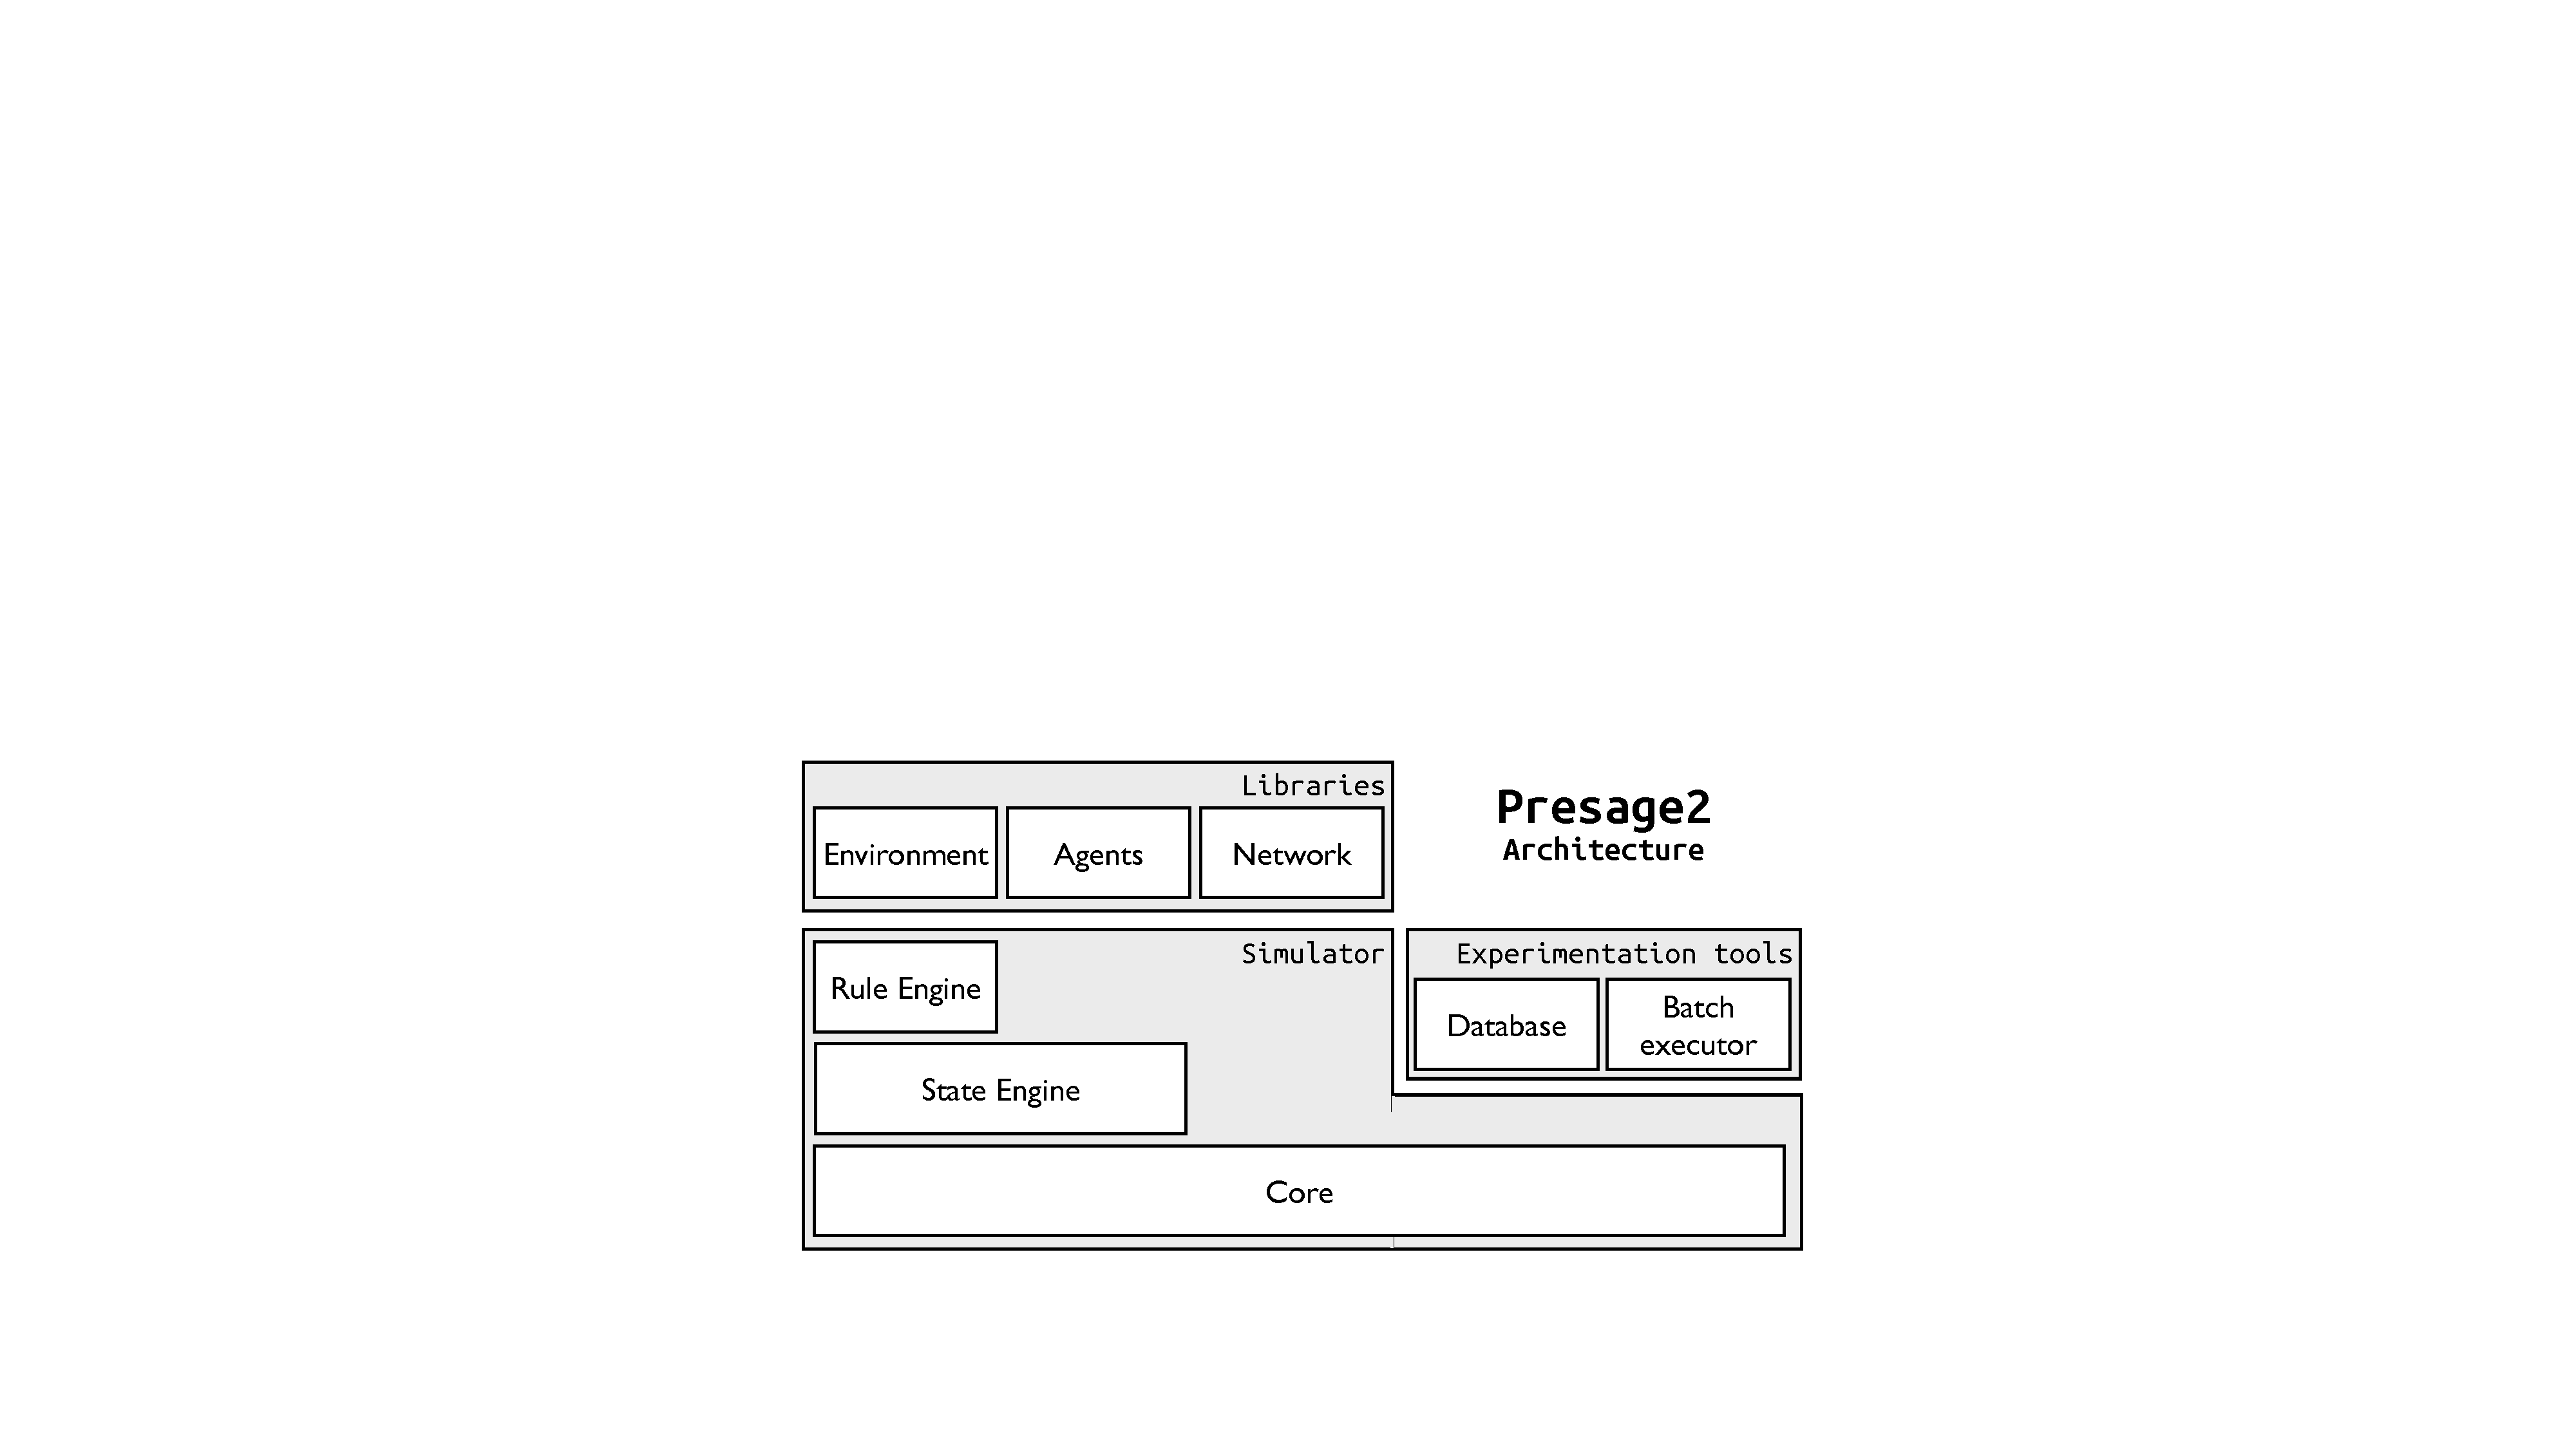
\includegraphics[width=\linewidth]{gfx/presage2/architecture_block}
\end{figure}

\subsection{Simulation initialisation}

With the state engine and simulation loop we have the base components to run a
simulation, however for this to work we need to initialise all the
components required for the simulation. Firstly, we must create all the required
objects for the environment: action handlers, environment functions and
environment services; secondly, we must create agents and link them to the
environment and environment services; and finally, we must create an initial
shared state of the environment and agents. This process should be easily
parameterised, as in order to perform experiments, we require that the initial state
can be easily controlled.

The construction of complex objects, with multiple dependencies, in languages
such as Java is often a verbose and tedious process, often referred to as 
`boilerplate' due to it requiring large quantities of code for little
functionality. In order to avoid needing such `boilerplate' we utilise a
practice called dependency injection~\citep{vanbrabant2008}. With this method
object dependencies are resolved at runtime, and the object tree is
automatically constructed according to \emph{bindings} specified by the user, with the
correct dependencies injected into each constructor. This allows us to specify
an environment with a series of \emph{bindings} which define which action
handlers, services etc.\ to load into the simulation. The dependencies for each of
these will also be automatically loaded.

% We will demonstrate the usefulness of this approach with two examples. Firstly,
% we can specify the set of action handlers, environment functions and environment
% services simply by just naming the classes we wish to load for each purpose.
% These classes will then be constructed automatically by the platform, providing 

Thus, an environment can be defined by declaring the set of classes which will
be action handlers, environment functions and environment services. This can
be done at runtime, and so be responsive to parameter changes. Simulation
parameters are also bound, enabling them to be injected at any point they are
needed. \autoref{alg:simspec} shows an example simulation specification in
Presage2. The \texttt{bind} and \texttt{agents} parameters are defined via
java annotations, and modules are used to define the environment and add
agents to it.

\begin{java}[caption={Specification of a simulation and parameters in Presage2},label=alg:simspec]
public class MySimulation extends RunnableSimulation {
	@Parameter
	public int size;

	@Parameter(optional=true)
	public int agents = 1;

	public void initialiseScenario(Scenario scenario) {
		addModule(Area.Bind.area2D(size, size));
		addModule(new AbstractEnvironmentModule()
			.addActionHandler(MoveHandler.class)
			.addParticipantEnvironmentService(ParticipantLocationService.class));

		for (int i = 0; i < agents; i++) {
			scenario.addAgent(new Agent(...));
		}
	}
}
\end{java}

The Presage2 platform allows for a simulation to specify a series of simulation
parameters. These are named variables which should be specified when executing a
simulation, and can take on any valid number, boolean, string, or enumerated
type value. These variables can be then used my the model implementer to control
the creation of initial agents and state. Agents are then connected to the
environment, through which they can attempt to load environment services they
require and perform actions.

\subsection{Module Library}

The intention of the software architecture we have chosen for the environment is
to enable a modular approach to environment modelling. These modules
compartmentalise particular functionalities such that they can be plugged into
any environment without conflict with other modules. In addition, modules
can build on top of other modules, providing high level abstractions. As a proof
of this design concept, and to provide the groundwork for a comprehensive set of
modules for common modelling tasks, we have implemented several environment
modules, which we present here.

\subsubsection*{Situated Agents}

A commonly used concept in \ac{ABM} is that of agents who are situated within a
physical environment. This is used in the modelling of scenarios where agents
must use their physical mobility to complete tasks and achieve goals. We provide
a module for this functionality.

The module provides environment services and an action handler for the
following:
\begin{itemize}
	\item Specifying a configurable area in which agents can move. This area may be
	continuous (any real number coordinate is valid within the area), or cellular 
	(agents may only occupy discrete cells). The area can also have each edge
	configured with a distinct behaviour for when an agent attempts to move beyond it,
	including stopping at the edge, wrapping around to the other side of the area,
	or simply throwing an exception. An environment service is provided for 
	querying information about the area.
	\item A location state which may be associated with an agent. This expresses
	the agent's current location within the environment area.
	\item An environment service for agents to query for their location and that of
	nearby agents. The results of the latter query may be limited if the agent has
	state to indicate a limited perception range.
	\item An action handler to process move actions from agents and update their
	location accordingly.
	\item Helper functions for agents to determine correct actions to move towards
	a target location and/or at certain speeds.
\end{itemize}

This implementation covers the majority of use-cases for situated agents.

\subsubsection*{Inter-agent communication}

We expressed the need for inter-agent communication in \autoref{sec:p2:reviewcritera}.
We implement a module which provides communication between agents via \emph{
message} actions. This module allows configuration of constraints which allow the
simulation of different dynamic network topologies. Arbitrarily complex
topologies can be simulated, but typical configurations would be fully
connected, peer-to-peer and mobile ad-hoc networks.

The network simulation is achieved by three entities:
\begin{itemize}
	\item The sending agent's interface to the network---This takes the set
	of messages it wishes to send and determines how to send them. For
	example in an ad-hoc network the user may wish to forward messages
	via a specific forwarding algorithm. 
	\item The message action handler---This takes messages which each agent
	wished to send and determines whether to send them based on a set
	of constraints. These reflect environmental constraints on messaging
	such as wireless range and/or random message loss.
	\item The receiving agent's network interface---This takes messages delivered
	from the global controller and decides what to do with them. This
	device may be forwarding messages in an ad-hoc network, dropping messages
	if it can't afford to forward them, or making messages intended for
	itself available to the underlying agent.
\end{itemize}

This architecture allows for flexible networks simulations and topology
constraints can be pushed to the appropriate level. For example if the user
wants to simulate an ad-hoc network but without having to write a specific
forwarding algorithm we can create a constraint in the global controller to
simulate how optimal forwarding would perform.

On top of this low level messaging we have built support for defining
messaging protocols as finite state machines. The user can specify
states and transitions, where moving to a state triggers a custom
action for the agent, and transitions are governed by composite rules
triggered by the arrival of messages. This framework allows complex
protocols to be defined and trivialises the often complex task of
managing multiple conversations with large numbers of agents simultaneously.

\subsubsection*{Social Capital}

\citet{Petruzzi2014} have developed a framework for social capital in agent-
based systems, based on the model of social capital proposed by
\citet{ostromahn2003}. This framework, shown in \autoref{fig:scf}, is
implemented for Presage2 as an agent module, allowing agents using it to
reason about social capital.

\begin{figure}[htb]
\caption[Social Capital Module]{Social Capital Module~\citep{Petruzzi2014}}
\label{fig:scf}
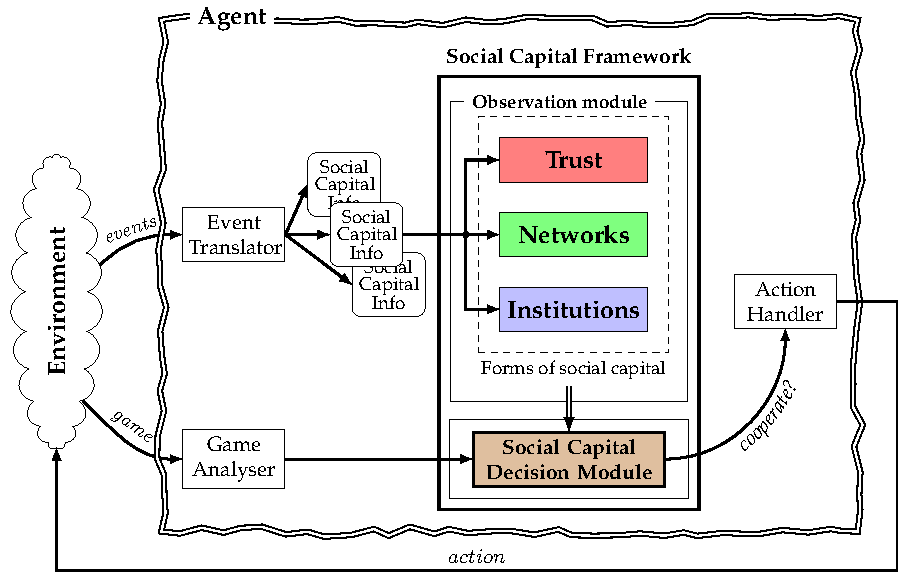
\includegraphics[width=\linewidth]{gfx/SCF2}
\end{figure}

\subsection{Rule Engine}

Rule- and logic-based specifications are a popular tool in artificial
intelligence. Equally, these tools can be used to formally specify complex
human decision processes~\citep{Pitt2005a}, and logic-based calculi such as
the Event Calculus~\citep{Kowalski1986} are commonly used for such
formalisations. For these reasons, we stated that a desirable feature for a
simulation platform would be rule-based specifications of the environment. To
this end, we have developed an extension to the Presage2 state engine to
incorporate a declarative rule-engine for management and modification of shared
state.

Production rules systems have a more simple reasoning engine than full logic
engines, but have been shown to be capable of implementing a useful subset of
logic programs~\citep{Bragaglia2012}. Thus by using such a rule engine we gain
the performance and scalability of production rules, while still being able to
implement rules translated from formal logics. Finally, the availability of rule
engines written in Java enables native integration between the rule engine and
simulation platform.

We have chosen to integrate the JBoss Drools business rule
engine\footnote{http://www.drools.org} into the Presage2 platform due to its
event processing and advanced reasoning features. The Drools rule engine
defines a \emph{knowledge base}, which is a repository of the defined rules,
and a \emph{working memory} which holds the current state of facts in the
current session. This \emph{working memory} can be modified by the user;
asserting, retracting and updating facts. The rules are not executed until the
rule-set is explicitly fired, at which point all rules in the \emph{knowledge
base} are checked and triggered.

This rule engine architecture maps directly to the Presage2 state engine
architecture. The \emph{working memory} can hold the simulation \emph{shared
state}, the rules perform the role of \emph{action handlers} and \emph{
environment services}, and triggering the rules performs a state change
transaction.

We provide an alternate state engine implementation which provides the same
features as the original, but using the rule-engine for state storage, and
with the addition of a rule-based state transition. Providing the same
interface as the default state engine ensures backwards compatibility for
environment modules. A subset of agent actions can be inserted directly into
the rule engine and then processed with rules.

\autoref{lst:ruleexample} shows an example of how a rule can implement action
handling. Rules are specified as `when \emph{condition} then
\emph{consequence}' clauses. The \emph{when} condition specifies that there
must be a \texttt{Move} action from an agent for whom there also exists a
\texttt{Location}. The colon represents a variable assignment or unification
to the name on the left-hand side of the operator. The \emph{then} clause
defines the consequence when a tuple matching the condition is found. In this
case the agent's location is updated and the action removed (to prevent
subsequent matches of the same rule).

\begin{drools}[caption={Drools rule example.},label=lst:ruleexample]
rule "Move agent"
    when
        $m : Move($a : agent, $dx : dx, $y : dy)
        $l : Location(agent == $a)
    then
        modify($l) {
            setX($l.getX() + $dx);
            setY($l.getY() + $dy);
        }
        retract($m);
end
\end{drools}

\subsection{Verification \& Validation}

Verification and Validation are important considerations when developing
software for scientific research. Verification is the process of checking if a
system is working as intended, while validation checks whether the system is
the correct system for the task~\citep{Wallace1989}. Specifically in the \ac{ABM}
domain,
verification covers whether the model is implemented
correctly, and validation concerns whether the model is the correct one~\citep{Ormerod2009}. 
From the perspective of a software tool for
simulation we must answer the following questions: How can we verify that the
software is executing the model correctly, and secondly, what does the tool
provide to aid verification and validation of models written with it?

The first question requires a verification of our implementation of the Presage2
framework. Using software testing we are able to guarantee, up to a high level of
confidence, that the framework implementation is correct. Tests range from unit
tests of individual classes or logical components, to full system integration
tests. Each test prepares an environment and inputs for the code under test. The
response to these stimuli are then compared to the expected values. These tests
are combined with an automated build system that will ensure that all tests pass
each time the platform is compiled. This prevents the introduction of errors
through later code modifications.

For example, a unit test may check that the vector addition used for computing
a new agent location given an initial location and movement action is
returning the correct results given a range of sample inputs. An integration
test would load an entire simulation and test whether the agent is able to
move as expected. The former test ensures that individual components are
implemented correctly, while the latter ensures the components are properly
composed and interact correctly.

The use of this unit-testing method in the platforms development has a knock-on
benefit for verification of user-defined models. With the platform's test-suite,
the groundwork is in place for addition of additional unit-testing of models.

However, verification in artificial intelligence and agent-based systems
introduces additional difficulties over general software
verification~\citep{Wooldridge1998}. \citet{Menzies2005} specify testing as a
baseline verification method, and go on to give four more advanced formal
methods: run-time monitoring, static analysis, model checking and theorem
proving. These methods can be applied to verify both environment and agent
implementations~\citep{Sudeikat2007a}.

Run-time monitoring is the analysis of the state of parts of an executing
program to detect invalid states. This can be achieved by logging within a
Java program. Further information can be provided by exceptions, which provide
traces to the occurrence of an error. Presage2 provides detailed logging through
the log4j library\footnote{http://logging.apache.org/log4j}, and also includes diagnostic simulation messages in the log
to allow one to ascertain when log messages are triggered in the simulation.
Furthermore, exceptions are caught and logged by the simulator, which will
provide information about expected and unexpected errors occurring during a
simulation.

Static analysis is error checking without code execution. Part of this can be
achieved using a strongly typed, compiled programming language, such as Java,
which will find coding errors at compile-time. This includes some errors
caused as a consequence of code changes leading to errors in other source
files. There are further tools providing in depth static analysis for Java
sources, such as FindBugs\footnote{http://findbugs.sourceforge.net} and
PMD\footnote{http://pmd.sourceforge.net}. These tools aim to detect common
programming errors, or problematic patterns. For Presage2, the use of a
language with a rich ecosystem of static analysis tools, Java, aids us in
regards to this kind of verification.

Model checking and theorem proving are more formal and stringent methods for
checking an algorithm and its implementation. Generally, these methods require
further consideration at design time about their integration. Model
checkers attempt to search all paths and states of a system to find property
violations. This requires finite and deterministic state, and a separate model
to describe the system to be checked. Therefore significant extra work is
required to take this approach.

Thus, the verification of an implemented model should be largely left to the
model implementer, but we do have tools to leave all options open. In
addition, in Presage2 we encourage design practices aimed at increasing the
robustness and reliability. Modularisation and component re-use attempts to
prevent individual components becoming overly complex. The Presage2 state
change framework also prevents non-determinism outside of the modeller's
control, for example the execution order of agents (which cannot be guaranteed
in multi-threaded execution) cannot lead to divergent states. Furthermore,
repeatable randomness is provided via the platform's pseudo random
number generation tools. Repeatability is an important aspect of
replicability~\citep{Axelrod1997,Ormerod2009}, so we encourage a best-practice
that the same input parameters and random seed combine to give identical
simulation results.

% Testing, Run-time monitoring, static analysis, model checking, theorum proving.
% Declarative specifications.
% Non-determinism: Concurrency - removed by framework; Environment, stochastic
% (Menzies2005)
% Ormderod2009 - verification (replication) vs validation

\subsection{Data gathering and visualisation}

A vital component of a simulation is being able to extract results after a run.
Results can range from a single value, or set of values, which summarise the final
state of the environment, to detailed raw data which could reconstruct the
simulation state at any time-step. With Presage2 our approach is to enable any
type of data to be stored, and in any quantity, depending on the user's
preference. This process should also be transparent to the simulation: if data
gathering is disabled the simulation will still run in the same way. Gathered
data should also always be associated with the input parameters to a simulation,
to ease the use of the platform for controlled experimentation.

Like MASON, and in contrast to Netlogo and Repast, Presage2 separates
visualisation from simulation. Visualisation is driven purely by gathered data,
in that rather than probing a running simulation in order to visualise we use
gathered and stored data. This approach allows real-time and post-simulation
analysis to be done using the same tools, when visualising we can always go back
as well as forward in time, and the simulation will always run at maximum speed.
The disadvantage is that we must explicitly state which data we wish to store
for visualisation and results may lag slightly behind the actual simulation
progress (though in practice simulations are likely to run faster than the speed
we want to view the visualisation).

Presage2 provides a high level data storage \ac{API}, allowing for storage of
data tuples. These tuples store data values associated with a named key, and may
also specify an agent and/or time-step for this data. Thus the following tuples
can be stored:
\begin{align*}
&(\mathtt{key},\mathtt{value})\\
&(\mathtt{key},\mathtt{t},\mathtt{value})\\
&(\mathtt{key},\mathtt{agent},\mathtt{value})\\
&(\mathtt{key},\mathtt{agent},\mathtt{t},\mathtt{value})
\end{align*}

This \ac{API} is paired with implementations for several popular storage
engines. These can be defined in configuration files such that the appropriate
database is loaded when the simulation starts. The current implementations
include the following:
\begin{itemize}
	\item JSON---Javascript Object Notation is a human-readable, machine parsable
	data-interchange format\footnote{http://json.org} which is supported by many
	programming languages. JSON data is stored in standard files so is easy to use
	with zero installation or configuration. This implementation is suitable for
	development or testing, however does not scale for significant volumes of data
	or allow concurrent data access.
	\item MongoDB\footnote{http://www.mongodb.org}---This is a fast document
	database. It is schema-less, and as such is naturally compatible with our tuple
	-based storage \ac{API}.
	\item SQL---This is a generic implementation for database which support SQL
	queries through the \ac{JDBC} \ac{API}. This includes popular \acp{DBMS} such
	as MySQL\footnote{http://www.mysql.com} and PostgreSQL\footnote{http://www.postgresql.org}.
\end{itemize}

Visualisation is then built either using the Presage2 \ac{API} directly in Java,
or using a preferred tool for the storage engine. The former is a more generic
approach, and we provide a framework for using this method for a web-based
simulation management and visualisation tool. 

\subsection{Experimental Support}

The usage of Presage2 for modelling and simulation can be expressed as a two
part process, as shown in \autoref{fig:presage2process}. In the design and
implementation phase decisions are made about the model and agent
implementations. A simulation specification is then created, combining 
user-implemented modules with modules from the Presage2 library in order to define
an environment, agents, and a mapping of parameters to initial state and
configuration. Following this, experimentation and evaluation can be performed
by providing parameter sets with a database configuration in order to generate
simulation data. This is an iterative process, as from initial data it is
likely that one will go back and refine the model and implementations in order
to fix problems and achieve a desired outcome. This process is enabled by
support for automated experiment generation and execution.

\begin{figure}
\centering
\caption{Presage2 simulation process diagram}\label{fig:presage2process}
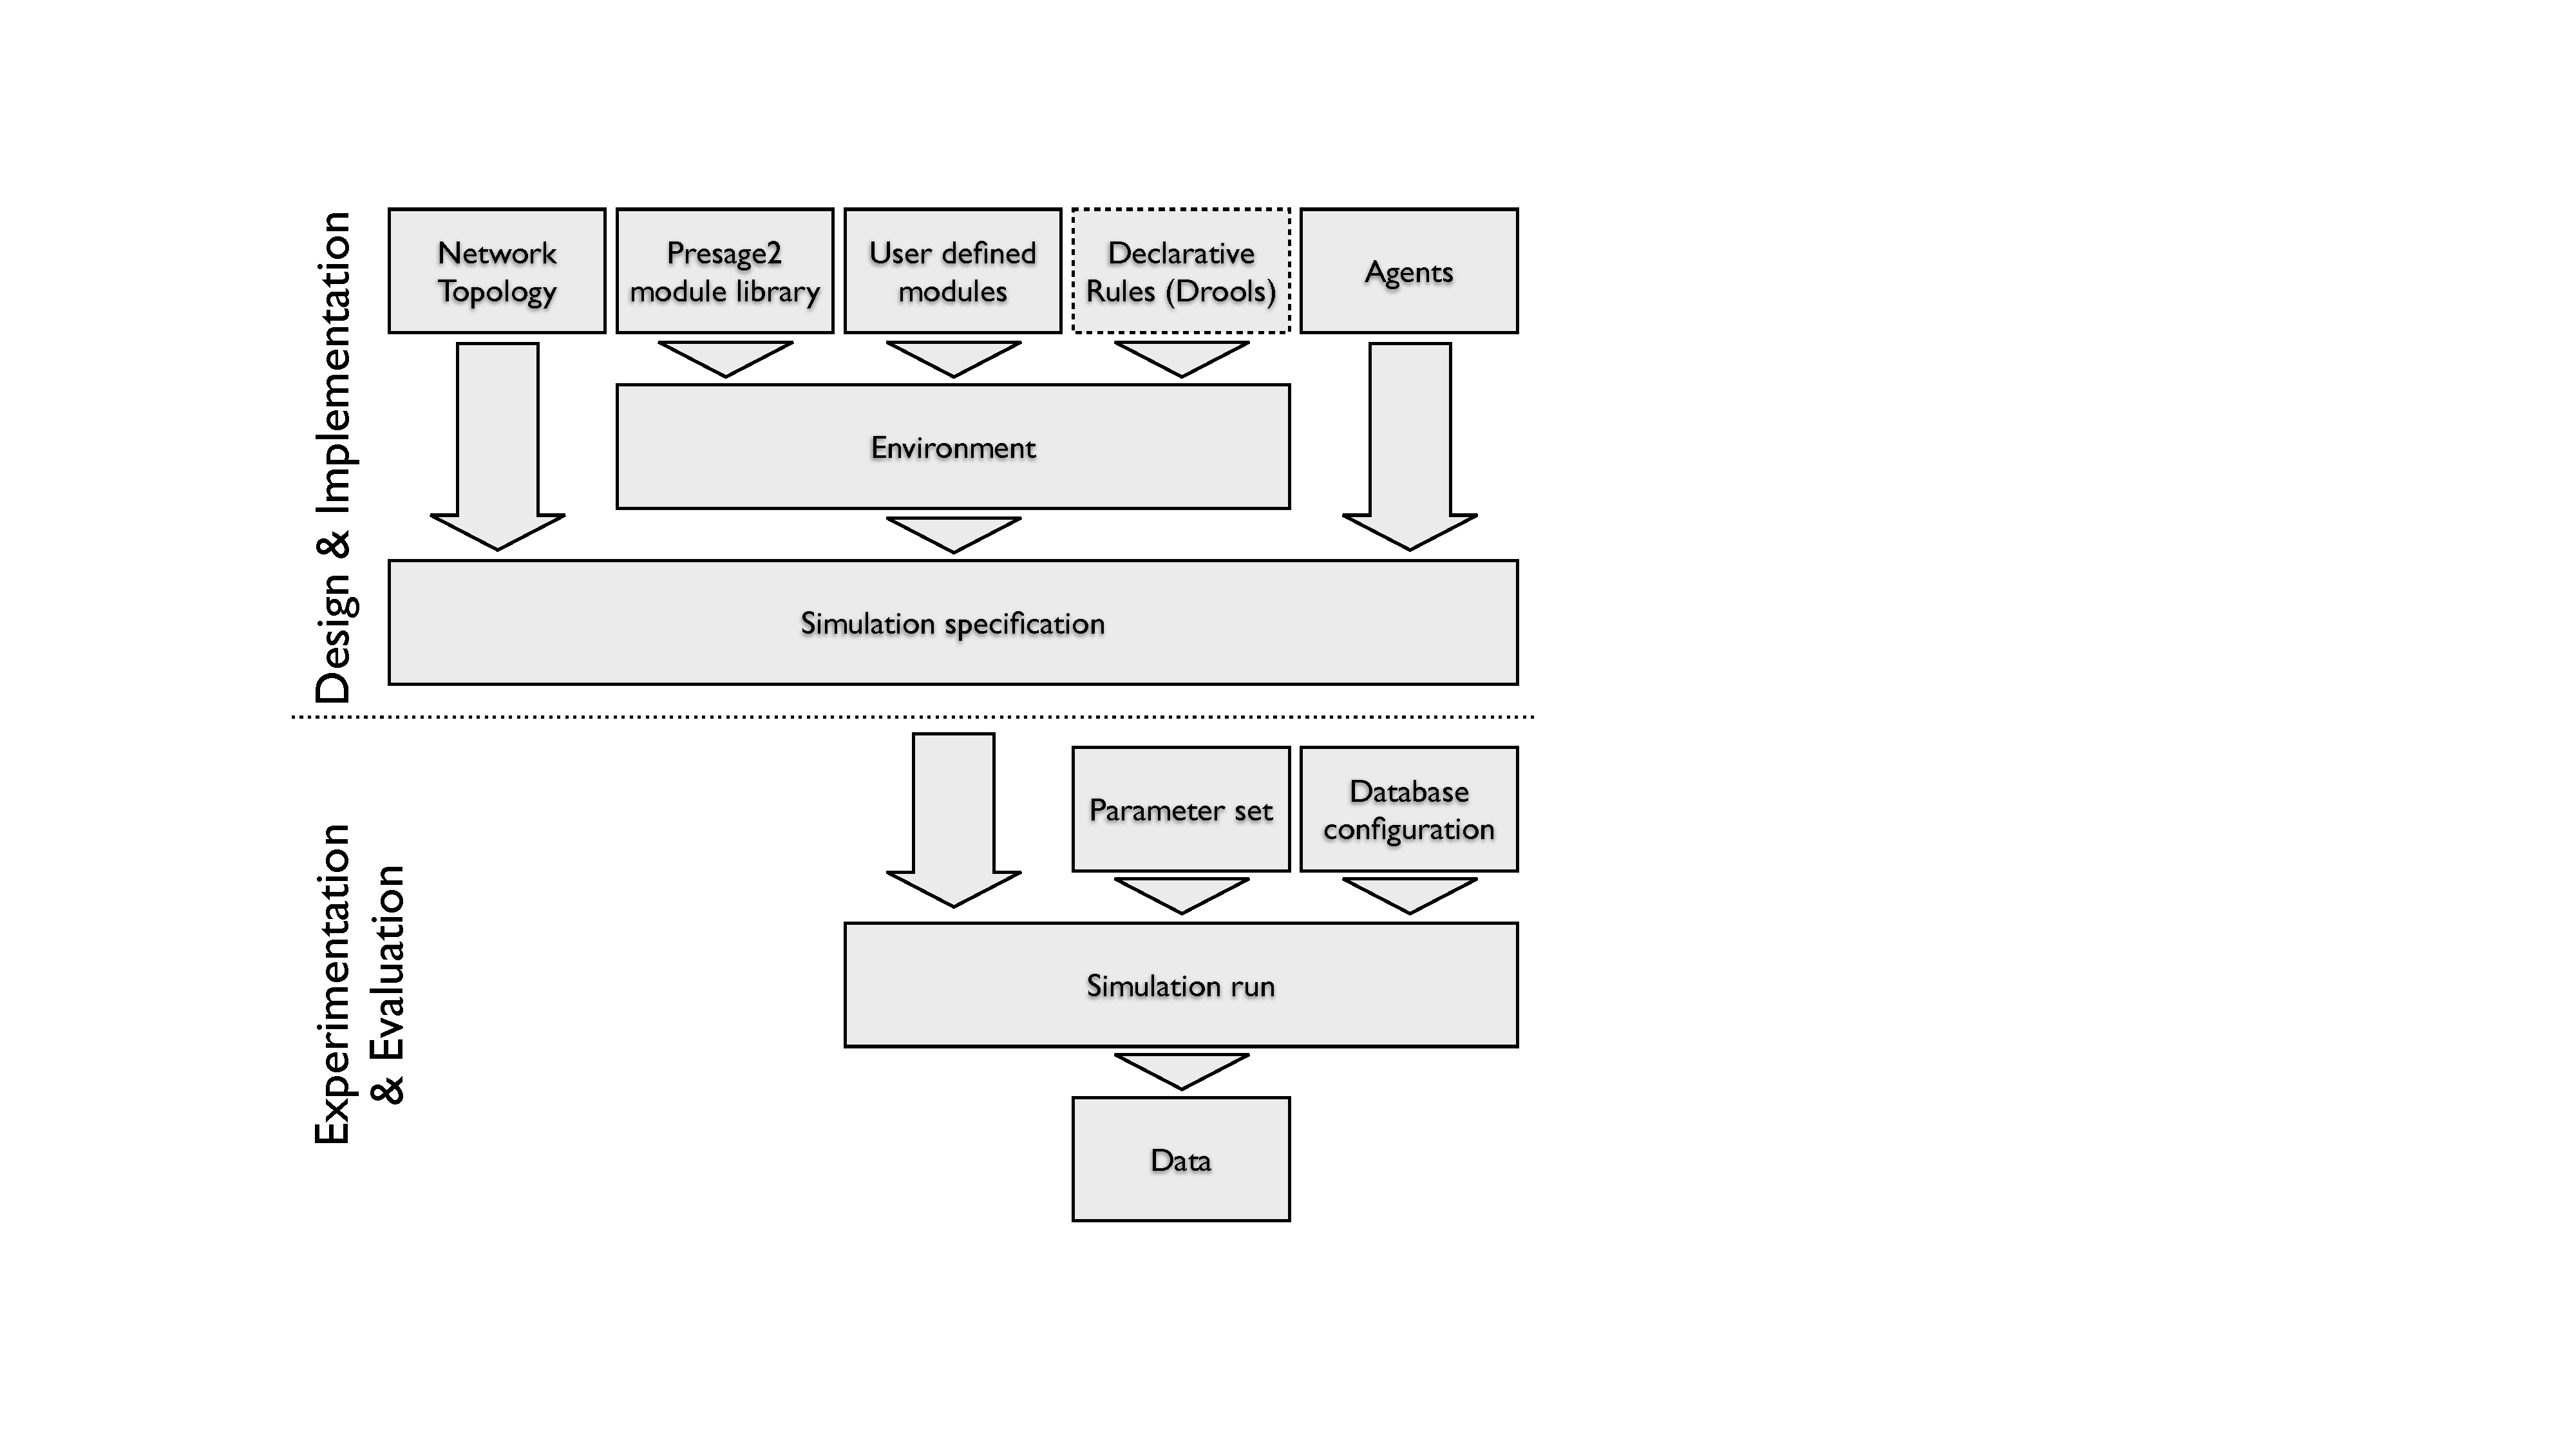
\includegraphics[width=0.8\linewidth]{gfx/presage2/simulation_process}
\end{figure}

We provide an \ac{API} for the specification of a set of values for each
parameter in the simulation. The tool can then automatically generate the set
of all parameter permutations, and create an experimental schedule from this
specification. The tool is also able to include a specified number of repeats
for each parameter set. Experimental schedules can then be run in batch by the
batch executor tool. This tool can be configured to exploit multiple machines
running experiments across a local area network, including using \ac{HPC}
facilities where available.

These simulation schedules can be managed through a web interface provided with
the platform. \autoref{fig:webuimanage} shows a screenshot of this interface
being used to add new simulations manually.

\begin{figure}
\caption{Simulation Management in Presage2 WebUI}\label{fig:webuimanage}
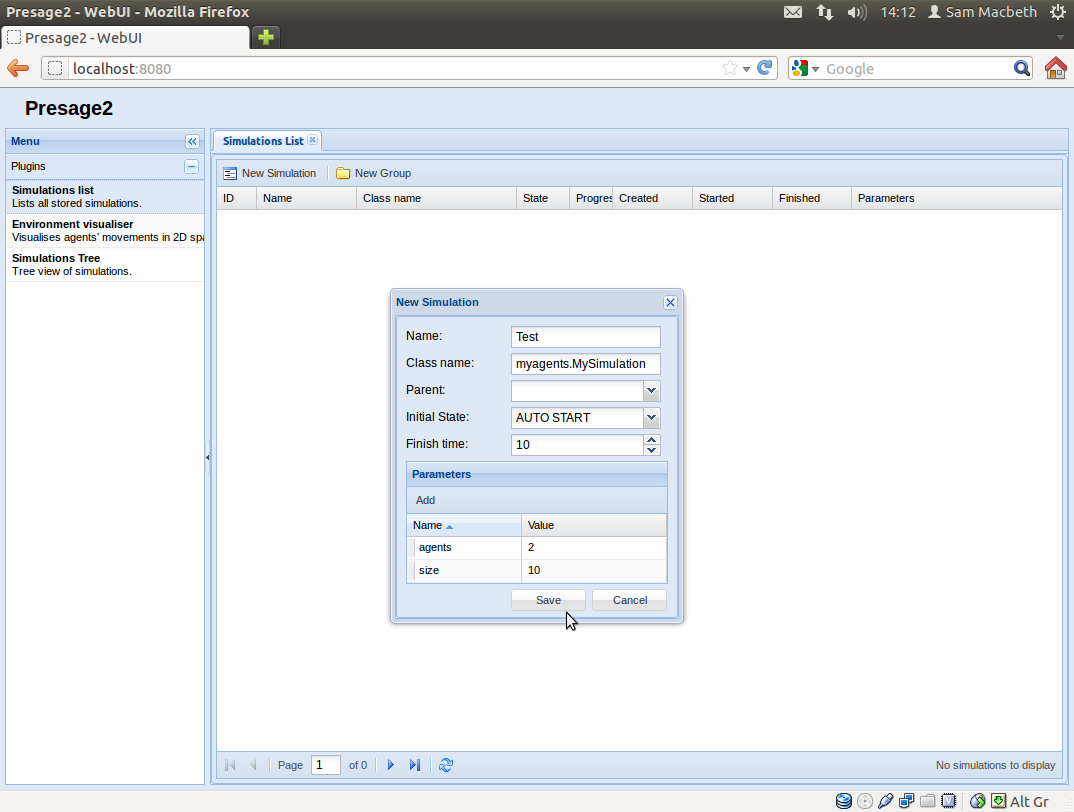
\includegraphics[width=\linewidth]{gfx/presage2/webui_manage}
\end{figure}

\section{Presage2 Showcase}

In this section we provide a short summary of a range of applications which have
been modelled and simulated using Presage2.\marginpar{Prose, subsection or
paragraph?}

Several applications have used Presage2 to model iterated games. In these
applications Presage2's time-driven model helps in particular to synchronise
each game round. Other applications model more concrete scenarios, such as
road networks, to apply agent-based modelling techniques to them. The final
set of applications have linked Presage2 to other tools, to provide on-demand
modelling for serious games or decision making:

\begin{itemize}
\item The LPG' game is a variant of a linear public good game, and was first defined
in \citet{Pitt2012c}. It has been used to explore the issue of non-compliance
in resource appropriation, and later to demonstrate a method of fairly
allocating resources based on Nicholas Rescher's theory of Distributive
Justice~\citep{Pitt2014}. The game was implemented using Presage2, utilising
the rule-engine to specify the game rules~\citep{Macbeth2012}.

This implementation of the LPG' game has been integrated with an Autonomous
Power Management system to apply Distributive Justice to the power grid~\citep{Kohler2014}.

\item The Game of Nomic, proposed by \citet{Suber1990}, is a rule amendment game.
The aim of the game is to successfully propose new rules, or modifications to
existing rules. A version of this game was implemented with Presage2, using
Drools for rule execution, to test if agents can successfully reason about
dynamic and mutable rule-sets~\citep{Holland2013}. This implementation
includes agents who are able to perform sub-simulations with the rule-set to
determine the effect of changes they intend to propose.

\item \citet{Petruzzi2014} test their social capital framework with a simple
cooperation game, implemented with Presage2.

\item \citet{Petruzzi2013} models a market for exchange of energy allocations
in a SmartGrid, utilising Social capital to encourage cooperation.

\item \citet{Schaumeier2013} models an exogenous common-pool resource, with
rules implemented to test each of \possessivecite{Ostrom1990} principles
for self-governing institutions. Again Drools was used for environmental
rules.

\item \citet{Sanderson2013} modelled fleets of self-driving cars, using
multiple self-adaptive mechanisms to optimise their behaviour. This work
included an implementation of Institutionalised Paxos
consensus~\citep{Sanderson2012} using Drools.

\item The Presage2 platform has been used to model the carbon emissions as a
common-pool resource, and exploring the effect of the Kyoto Protocol on these
emissions~\citep{Macbeth2014}. This work provides an example case of 
policy-based modelling with Presage2.

\item The Social Mpower game is a Serious game to inform, raise awareness and motivate
consumers of energy efficiency~\citep{Bourazeri2014}. Presage2 is used as a
background simulation component of the game, communicating with a graphical game
frontend, which sends actions triggered by both humans playing the game and
computational agents within the game.
% TODO cite PRIMA later.
\end{itemize}

\section{Presage2 Evaluation \& Conclusion}

Having described the Presage2 platform and its usage, we return to our
evaluative criteria from \autoref{sec:p2:review} in order to evaluate how
well Presage2 performs as a platform for principled operationalisation of 
socio-technical systems.

\autoref{tab:presagereview} shows Presage2 evaluated according to the basic
criteria. Like the other Java-based simulation platforms, we require strong
programming skills. However, the introduction of rule-based components allows
for these parts to be easier to understand for non-programmers than standard
Java code. So far the platform has not given significant focus to integration of
graphing and visualisation options, instead taking a data-driven approach and
letting users choose their preferred data-visualisation tool. Finally, tutorials
and documentation are readily available from the Presage2 webpage\footnote{http
://www.presage2.info}.

\begin{table}[h]
\begin{minipage}{1\textwidth}
	\myfloatalign
	\caption{Evaluation of Presage2 according to review criteria}\label{tab:presagereview}
	\begin{tabularx}{\textwidth}{X|X}
	Criterion & Presage2 \\ \midrule
	Programming Language & Java \\
	Software License & LGPL\footnote{Lesser General Public License: \ac{GPL}
	compatible licence for software libraries.} \\
	Required programming experience & Strong \\
	Integrated graphics & Some \\
	Tutorials / Documentation & Yes \\
	\end{tabularx}
\end{minipage}
\end{table}

Presage2 has limited \ac{GUI} tools, thus support for modelling remains limited.
The tools that it does have mainly support experimentation, with a \ac{GUI} for
management of simulation runs, automated simulation generation, distributed
experiment execution, and detailed data recording.

Large numbers of complex agents can be run due to the simulator's exploitation
of multi-threaded execution, and the agent agnostic approach allowing for users
to implement complex agents in simulations. These agents can also be
automatically generated from input parameters as part of the initial state of
the simulation.

The Presage2 state engine enables simulation of situated agents;
automatically generated, dynamic networks; and dynamically changing models.
Furthermore, these features are modular, and separated from agent
implementations.

Therefore, we believe that the Presage2 platform is not only an improvement over
the original Presage platform, but has several significant features which
distinguish it as a tool for principled operationalisation over the platforms we
have reviewed in \autoref{sec:p2:review}. The remaining outstanding issue, with
respect to our criteria, is that of graphical modelling support.

Such graphic modelling support is a topic of future platform development. We are
confident that graphical support can be added to the platform without
sacrificing the current functionality and performance, and without the resultant
graphical tool being too limited for generation of complex models. In
particular, three properties of Presage2 will aid this. Firstly, the platform's
modularity allows for design by composition. An environment can be built by
simply combining a set of modules and linking simulation parameters to module
parameters. Secondly, the Java language's introspective and self generation
capabilities will enable automatic code generation from graphical models.
Therefore the graphical tool will simply act as a compiler to generate Presage2
models, and no functionality is lost. Finally, through the Eclipse IDE\footnote{
http://eclipse.org}, Java has significant support for interactive graphical
tools for code generation. We envisage that by leveraging these features we can
bring graphical model development to Presage2.

The use of the platform over a range of projects has shown its effectiveness
as a simulation and modelling tool. The focus of the current applications on
situations with a strong rule or governance mechanic is largely due to the
uptake of the platform. It has been adopted in this domain due to the ease of
working with rule-based specifications and implementing adaptive and self-
organising agents. However, we have shown in this chapter that the platform's
framework is generic and extendible. Thus, we expect an increase in application
domains for which Presage2 is used as it gains traction.



%A single time-step consists of running the state observability function to determine the data available for each agent, running each agent function, then running the state transformer function with the aggregated agent actions. This specifies a simple and easy to parallelise simulation loop. The shared state is constant until the final step, thus there are no issues with mutable state or shared memory management. We can further optimise by decomposing the state transformer function into three components:
%\begin{itemize}
%\item A set of \emph{action handler} functions to define a state change as a result of an agent action. Different functions may be applicable to different action types or under different conditions.
%\item A set of \emph{environment} functions which define state changes purely from the current shared state. This may be persistent effects on agents (e.g.\ momentum), periodic (either random or triggered) events, etc.
%\item A function to define how to apply the state changes generated by the functions above to the state.
%\end{itemize}
%
%This distinction allows us to maximise the parallisable part of the simulation loop, leaving simply a atomic state transition to be executed at the end of the time-step. Thus the simulation loop entails the collection and execution of all agent and environment functions (in parallel when hardware allows). Once this process completes we can execute a state transition.
%
%In this simulation loop description we have omitted the state observability function. The simulation loop simply acts as a multi-threaded scheduler, executing the functions as described above each time-step. State is handled by a state engine. This engine holds the

% Simulation loop
% State engine
% Modularity: Action handlers, Environment services
% Agents/Environment
% Modules: 
% Simulation parameterisation
% Boilerplate: Guice

%\subsection{Implementation}
%
%The Presage2 platform is implemented as a Java library. \autoref{fig:presage2block} shows the various components which make up the platform as a whole. In this section we describe the implementation specifics of these components.



%\subsubsection*{State Engine}
%
%The state engine implements the core of the Presage2 framework, allowing for the definition of an environment and the observability of shared state. 
%
%Access to raw shared state is provided through the \texttt{EnvironmentSharedStateAccess} interface, which defines functions for creation, modification and retrieval of state values. State can either be associated with an agent or the environment, and is addressed with a string key. State values can be any serializable object\footnote{In Java this simply means that it is possible to save the object to, and load it from, a string representation.}. The implementations of this interface implement a super interface \texttt{SharedStateStorage} which adds an additional function which the simulator uses to commit a state change transaction.
%
%Through the shared state interface state changes can be defined simply by specifying a new value for a given state key. However, this method is non-deterministic in the case when there are multiple state changes for the same key in one transaction. Therefore the preferred method, provided by the same interface, is to specify a \texttt{StateTransformer} object. This class defines a function which returns a new state value based on the current value. In the case with multiple updates of the same state this function will be able to work with an intermediate state value during the transaction.
%
%\begin{lstlisting}[caption=\texttt{StateTransformer} example,language=Java]
%// EnvironmentSharedStateAccess sharedState
%sharedState.change(key, agentId, new StateTransformer() {
%	public Serializable transform(Serializable state) {
%		Integer current = (Integer) state;
%		return current + 1;
%	}
%});
%\end{lstlisting}
%
%\emph{Action Handlers}, \emph{environment functions} and \emph{environment services} are built on top of this base shared state. 

%The default \texttt{SharedStateStorage} implementation simply uses a Java \texttt{Map} to store state information.
%
%\subsubsection*{Core}
%
%This component controls and executes the main simulation loop and core functions. 

% Distribution: Maven + git


% Environment requirements
% Agent requirements

%Executable specifications such as the Event Calculus~\citep{Kowalski1986} can even eliminate this step by being both formal representation and computer model~\citep{Artikis2010}. However this approach has limitations in scalability and its ability to span the entire system specification.